\subsection{Formato de representación de las figuras}

\todo{Añadir el diagrama y hacer referencia a el cuando una explicación textual no sea suficiente}
Las imágenes vienen representadas por un documento XML  estructurado de la siguiente manera:

\begin{itemize}
\item \textbf{Shapes}: Representa la imagen completa, contiene un listado de las figuras resultantes del análisis.
\item \textbf{Figure}: Contiene la información relativa a una figura.
\item \textbf{Id}: Identificador único de la figura.
\item \textbf{Color}: Identificador para delimitar la información sobre el color.
\item \textbf {RGB}: Identificador para delimitar la información sobre los valores RGB del color.
\item \textbf{R}: Valor referente a la escala de rojo en la escala RGB.
\item \textbf{G}: Valor referente a la cantidad de verde en la escala RGB.
\item \textbf{B}: Valor referente a la cantidad de azul presente en escala RGB.
\item \textbf{VertexList}: Lista de vértices que componen el polígono.
\item \textbf{Vertex [type=``normal'']}: Identificador para delimitar un vértice que pertenece a uno de los extremos de una recta o curva del polígono.
\item \textbf{Position}: Identificador para delimitar la posición de un vértice en la imagen.
\item \textbf{X}: Componente x de la posición del vértice.
\item \textbf{Y}: Componente y de la posición del vértice.
\item \textbf{Vertex [type=``center'']}: Identificador para delimitar un vértice que señala el centro de circunferencia que forma la curva que conecta el vértice anterior a este con el siguiente.
\item \textbf{Area}: Valor numérico del área de una figura.
\item \textbf{Canvas}: Identificador que delimita las figuras situadas dentro de la figura que contiene este elemento. 
\end{itemize}

\subsection{Formato de representación de música}

\todo{Repasar formalizar}

La estructura para representar la música propuesta en el proyecto está determinada por un árbol que trabaja desde el elemento más general, la canción que se va a componer, al más específico, cada una de las notas que componen dicha canción, como muestra la Figura~\ref{fig:structmusic}.\\
	
	\begin{figure}[htbp]
	\centering
	\hspace*{-0.1in}
	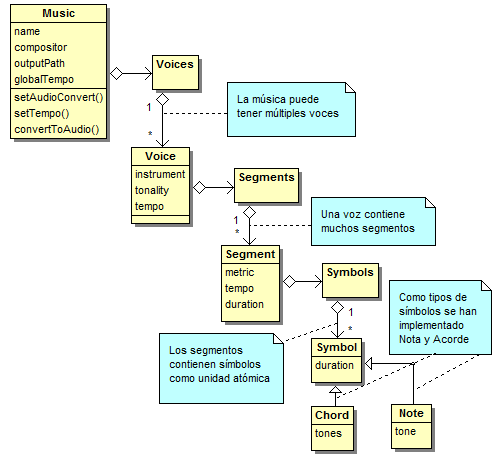
\includegraphics[scale=0.47]{graphics/musica-estructura.png}
	\caption{Estructura de una pieza musical}
	\label{fig:structmusic}
	\end{figure}


\textbf{Música}: Al nivel de la Música, trabajamos con la información relativa a toda la canción que se va a componer, por un lado está información relativa al nombre de la composición y del compositor que la ha hecho, también dispone de una serie de voces a partir de las cuales estará formada la canción y su tempo. Por último a un nivel más cercano, la implementación permitirá elegir con que herramienta querremos crear el archivo de audio de salida.
\newline

\textbf{Voz}: Por debajo de la Música se trabaja con las Voces. Su estructura permite determinar el instrumento, la tonalidad y el tempo de cada una de las voces que componen una pieza, cada una de estas voces esta compuesta de varios segmentos musicales, los cuales al ser reproducidos en el orden establecido por el compositor forman la Voz en cuestión.
\newline

\textbf{Segmento}: Estos elementos tienen la posibilidad de establecer su propia métrica, su tempo y su duración. Los segmentos a su vez están formados por una sucesión de símbolos.
\newline

\textbf{Símbolo}: Son la unidad a partir de la cual se crean todos los elementos básicos de la música, símbolo nos permite establecer una duración para estos elementos. Actualmente el proyecto crea dos tipos de elementos a partir de símbolo:
\begin{itemize}
\item \textbf{Notas}: Estos símbolos tienen asociada una duración, determinada por el componente anterior, y un tono establecido por un número que posteriormente será interpretado con la herramienta que generará el archivo de audio.
\item \textbf{Acordes}: Los acordes están formados de la misma manera que las notas pero en lugar de tener asociado un único tono pueden tener de dos a tres tonos diferentes, en la práctica esto resultará en todos los tonos sonando a la vez durante el mismo tiempo una vez generada la canción.
\end{itemize}
 
